% Options for packages loaded elsewhere
\PassOptionsToPackage{unicode}{hyperref}
\PassOptionsToPackage{hyphens}{url}
%
\documentclass[
]{article}
\usepackage{amsmath,amssymb}
\usepackage{iftex}
\ifPDFTeX
  \usepackage[T1]{fontenc}
  \usepackage[utf8]{inputenc}
  \usepackage{textcomp} % provide euro and other symbols
\else % if luatex or xetex
  \usepackage{unicode-math} % this also loads fontspec
  \defaultfontfeatures{Scale=MatchLowercase}
  \defaultfontfeatures[\rmfamily]{Ligatures=TeX,Scale=1}
\fi
\usepackage{lmodern}
\ifPDFTeX\else
  % xetex/luatex font selection
\fi
% Use upquote if available, for straight quotes in verbatim environments
\IfFileExists{upquote.sty}{\usepackage{upquote}}{}
\IfFileExists{microtype.sty}{% use microtype if available
  \usepackage[]{microtype}
  \UseMicrotypeSet[protrusion]{basicmath} % disable protrusion for tt fonts
}{}
\makeatletter
\@ifundefined{KOMAClassName}{% if non-KOMA class
  \IfFileExists{parskip.sty}{%
    \usepackage{parskip}
  }{% else
    \setlength{\parindent}{0pt}
    \setlength{\parskip}{6pt plus 2pt minus 1pt}}
}{% if KOMA class
  \KOMAoptions{parskip=half}}
\makeatother
\usepackage{xcolor}
\usepackage[margin=1in]{geometry}
\usepackage{color}
\usepackage{fancyvrb}
\newcommand{\VerbBar}{|}
\newcommand{\VERB}{\Verb[commandchars=\\\{\}]}
\DefineVerbatimEnvironment{Highlighting}{Verbatim}{commandchars=\\\{\}}
% Add ',fontsize=\small' for more characters per line
\usepackage{framed}
\definecolor{shadecolor}{RGB}{248,248,248}
\newenvironment{Shaded}{\begin{snugshade}}{\end{snugshade}}
\newcommand{\AlertTok}[1]{\textcolor[rgb]{0.94,0.16,0.16}{#1}}
\newcommand{\AnnotationTok}[1]{\textcolor[rgb]{0.56,0.35,0.01}{\textbf{\textit{#1}}}}
\newcommand{\AttributeTok}[1]{\textcolor[rgb]{0.13,0.29,0.53}{#1}}
\newcommand{\BaseNTok}[1]{\textcolor[rgb]{0.00,0.00,0.81}{#1}}
\newcommand{\BuiltInTok}[1]{#1}
\newcommand{\CharTok}[1]{\textcolor[rgb]{0.31,0.60,0.02}{#1}}
\newcommand{\CommentTok}[1]{\textcolor[rgb]{0.56,0.35,0.01}{\textit{#1}}}
\newcommand{\CommentVarTok}[1]{\textcolor[rgb]{0.56,0.35,0.01}{\textbf{\textit{#1}}}}
\newcommand{\ConstantTok}[1]{\textcolor[rgb]{0.56,0.35,0.01}{#1}}
\newcommand{\ControlFlowTok}[1]{\textcolor[rgb]{0.13,0.29,0.53}{\textbf{#1}}}
\newcommand{\DataTypeTok}[1]{\textcolor[rgb]{0.13,0.29,0.53}{#1}}
\newcommand{\DecValTok}[1]{\textcolor[rgb]{0.00,0.00,0.81}{#1}}
\newcommand{\DocumentationTok}[1]{\textcolor[rgb]{0.56,0.35,0.01}{\textbf{\textit{#1}}}}
\newcommand{\ErrorTok}[1]{\textcolor[rgb]{0.64,0.00,0.00}{\textbf{#1}}}
\newcommand{\ExtensionTok}[1]{#1}
\newcommand{\FloatTok}[1]{\textcolor[rgb]{0.00,0.00,0.81}{#1}}
\newcommand{\FunctionTok}[1]{\textcolor[rgb]{0.13,0.29,0.53}{\textbf{#1}}}
\newcommand{\ImportTok}[1]{#1}
\newcommand{\InformationTok}[1]{\textcolor[rgb]{0.56,0.35,0.01}{\textbf{\textit{#1}}}}
\newcommand{\KeywordTok}[1]{\textcolor[rgb]{0.13,0.29,0.53}{\textbf{#1}}}
\newcommand{\NormalTok}[1]{#1}
\newcommand{\OperatorTok}[1]{\textcolor[rgb]{0.81,0.36,0.00}{\textbf{#1}}}
\newcommand{\OtherTok}[1]{\textcolor[rgb]{0.56,0.35,0.01}{#1}}
\newcommand{\PreprocessorTok}[1]{\textcolor[rgb]{0.56,0.35,0.01}{\textit{#1}}}
\newcommand{\RegionMarkerTok}[1]{#1}
\newcommand{\SpecialCharTok}[1]{\textcolor[rgb]{0.81,0.36,0.00}{\textbf{#1}}}
\newcommand{\SpecialStringTok}[1]{\textcolor[rgb]{0.31,0.60,0.02}{#1}}
\newcommand{\StringTok}[1]{\textcolor[rgb]{0.31,0.60,0.02}{#1}}
\newcommand{\VariableTok}[1]{\textcolor[rgb]{0.00,0.00,0.00}{#1}}
\newcommand{\VerbatimStringTok}[1]{\textcolor[rgb]{0.31,0.60,0.02}{#1}}
\newcommand{\WarningTok}[1]{\textcolor[rgb]{0.56,0.35,0.01}{\textbf{\textit{#1}}}}
\usepackage{graphicx}
\makeatletter
\def\maxwidth{\ifdim\Gin@nat@width>\linewidth\linewidth\else\Gin@nat@width\fi}
\def\maxheight{\ifdim\Gin@nat@height>\textheight\textheight\else\Gin@nat@height\fi}
\makeatother
% Scale images if necessary, so that they will not overflow the page
% margins by default, and it is still possible to overwrite the defaults
% using explicit options in \includegraphics[width, height, ...]{}
\setkeys{Gin}{width=\maxwidth,height=\maxheight,keepaspectratio}
% Set default figure placement to htbp
\makeatletter
\def\fps@figure{htbp}
\makeatother
\setlength{\emergencystretch}{3em} % prevent overfull lines
\providecommand{\tightlist}{%
  \setlength{\itemsep}{0pt}\setlength{\parskip}{0pt}}
\setcounter{secnumdepth}{-\maxdimen} % remove section numbering
\ifLuaTeX
  \usepackage{selnolig}  % disable illegal ligatures
\fi
\usepackage{bookmark}
\IfFileExists{xurl.sty}{\usepackage{xurl}}{} % add URL line breaks if available
\urlstyle{same}
\hypersetup{
  pdftitle={Indonesia's Tree Cover Loss},
  pdfauthor={asg2425},
  hidelinks,
  pdfcreator={LaTeX via pandoc}}

\title{Indonesia's Tree Cover Loss}
\author{asg2425}
\date{2024-11-28}

\begin{document}
\maketitle

\subsection{Background}\label{background}

Indonesia boasts the third largest forest in the world, home to a rich
biodiversity ecosystem (Greenpeace, n.d.). However, recent news suggests
that big corporations are planning to remove the forest in Papua, where
indigenous people depend on and protect its natural resources, to make
way for palm oil plantations (Greenpeace Southeast Asia, 2024). This
news raises questions about the current condition of Indonesia's forest
and how it has changed over the years.

\subsection{Data Source}\label{data-source}

To address my concerns, I found the Global Forest Watch (GFW) website
that provides data on Indonesia's annual tree cover loss from 2001-2023.
The data is accessible via the following link:
\url{https://www.globalforestwatch.org/dashboards/country/IDN/?category=land-cover&location=WyJjb3VudHJ5IiwiSUROIl0\%3D&map=eyJjYW5Cb3VuZCI6dHJ1ZX0\%3D}.

The data was generated by the University of Maryland's GLAD laboratory
in collaboration with Google (Hansen et al.~2013). GFW refers tree cover
loss as a ``stand replacement disturbance'' that entails at minimum of
50\% tree cover removal within a 30-meter pixel. I selected two sheets
from the Excel file that display the tree cover data: Country tree cover
loss and Subnational 1 tree cover loss.

The following are the descriptions of each sheet from the GFW data:
Country tree cover loss: Hectares of tree cover loss at a national
level, between 2001-2023, categorized by percent canopy cover in 2000.
Subnational 1 tree cover loss: Hectares of tree cover loss at the first
sub-national level, between 2001-2023, categorized by percent canopy
cover in 2000.

Note: Canopy cover (CC) is the percentage of ground that individual tree
crowns cover. This is measured based on the vertical projection of the
tree crown's perimeter onto a horizontal plane (van Laar and Akça,
2007). A 100\% CC indicates that the area is fully covered, whereas a
0\% CC indicates a canopy gap, basic open area, or forest opening that
allows sunlight to reach plants that may grow closer to the ground
(Vatandaslar et al., 2024).

\subsection{Research Question}\label{research-question}

From examining the sheets, I developed two research questions, which
are: *** 1. What are the magnitudes of tree cover loss per year in
Indonesia from 2001 to 2023?*** *** 2. What are the magnitudes of tree
cover loss per year in each province from 2001 to 2023?***

\subsection{Data Preparation}\label{data-preparation}

Since the data are in wide format on both sheets, I converted them to
long format and input the year as a factor before visualising it. GFW
uses the 30\% canopy cover threshold as a default for analysis, so I
filtered the tree cover loss numbers within this threshold for the
`Subnational 1 tree cover loss' data.

\begin{Shaded}
\begin{Highlighting}[]
\DocumentationTok{\#\# install packages for data preparation \#\#}
\FunctionTok{install.packages}\NormalTok{(}\StringTok{"readxl"}\NormalTok{)}
\FunctionTok{install.packages}\NormalTok{(}\StringTok{"writexl"}\NormalTok{)}
\FunctionTok{install.packages}\NormalTok{(}\StringTok{"reshape2"}\NormalTok{)}
\FunctionTok{install.packages}\NormalTok{(}\StringTok{"dplyr"}\NormalTok{)}

\DocumentationTok{\#\# install packages to make scatter plot) \#\#}
\FunctionTok{install.packages}\NormalTok{(}\StringTok{"ggplot2"}\NormalTok{)}
\FunctionTok{install.packages}\NormalTok{(}\StringTok{"RColorBrewer"}\NormalTok{)}

\DocumentationTok{\#\# install a package to make interactive plot \#\#}
\FunctionTok{install.packages}\NormalTok{(}\StringTok{"plotly"}\NormalTok{)}
\end{Highlighting}
\end{Shaded}

\begin{Shaded}
\begin{Highlighting}[]
\CommentTok{\#set directory \% load the packages}
\FunctionTok{library}\NormalTok{(here)}
\FunctionTok{library}\NormalTok{(readxl)}


\CommentTok{\#import data from excel \& promtply check the data using head() function}
\NormalTok{country\_tc\_loss\_wide }\OtherTok{\textless{}{-}} \FunctionTok{read\_excel}\NormalTok{(}\StringTok{"IDN.xlsx"}\NormalTok{, }\AttributeTok{sheet =} \StringTok{"Country tree cover loss"}\NormalTok{)}
\FunctionTok{head}\NormalTok{(country\_tc\_loss\_wide)}
\end{Highlighting}
\end{Shaded}

\begin{verbatim}
## # A tibble: 6 x 29
##   country   threshold  area_ha extent_2000_ha extent_2010_ha `gain_2000-2020_ha`
##   <chr>         <dbl>    <dbl>          <dbl>          <dbl>               <dbl>
## 1 Indonesia         0   1.89e8      189024469      189024469             4882138
## 2 Indonesia        10   1.89e8      165098735      162774273             4882138
## 3 Indonesia        15   1.89e8      163637823      160772132             4882138
## 4 Indonesia        20   1.89e8      162782759      160094820             4882138
## 5 Indonesia        25   1.89e8      161883473      158971104             4882138
## 6 Indonesia        30   1.89e8      160641223      157793272             4882138
## # i 23 more variables: tc_loss_ha_2001 <dbl>, tc_loss_ha_2002 <dbl>,
## #   tc_loss_ha_2003 <dbl>, tc_loss_ha_2004 <dbl>, tc_loss_ha_2005 <dbl>,
## #   tc_loss_ha_2006 <dbl>, tc_loss_ha_2007 <dbl>, tc_loss_ha_2008 <dbl>,
## #   tc_loss_ha_2009 <dbl>, tc_loss_ha_2010 <dbl>, tc_loss_ha_2011 <dbl>,
## #   tc_loss_ha_2012 <dbl>, tc_loss_ha_2013 <dbl>, tc_loss_ha_2014 <dbl>,
## #   tc_loss_ha_2015 <dbl>, tc_loss_ha_2016 <dbl>, tc_loss_ha_2017 <dbl>,
## #   tc_loss_ha_2018 <dbl>, tc_loss_ha_2019 <dbl>, tc_loss_ha_2020 <dbl>, ...
\end{verbatim}

\begin{Shaded}
\begin{Highlighting}[]
\NormalTok{subnational\_tc\_loss\_wide }\OtherTok{\textless{}{-}} \FunctionTok{read\_excel}\NormalTok{(}\StringTok{"IDN.xlsx"}\NormalTok{, }\AttributeTok{sheet =} \StringTok{"Subnational 1 tree cover loss"}\NormalTok{)}
\FunctionTok{head}\NormalTok{(subnational\_tc\_loss\_wide)}
\end{Highlighting}
\end{Shaded}

\begin{verbatim}
## # A tibble: 6 x 30
##   country   subnational1 threshold area_ha extent_2000_ha extent_2010_ha
##   <chr>     <chr>            <dbl>   <dbl>          <dbl>          <dbl>
## 1 Indonesia Aceh                 0 5683651        5683651        5683651
## 2 Indonesia Aceh                10 5683651        5090908        4996300
## 3 Indonesia Aceh                15 5683651        5050170        4946857
## 4 Indonesia Aceh                20 5683651        5029129        4932164
## 5 Indonesia Aceh                25 5683651        5014672        4908703
## 6 Indonesia Aceh                30 5683651        4984710        4879170
## # i 24 more variables: `gain_2000-2020_ha` <dbl>, tc_loss_ha_2001 <dbl>,
## #   tc_loss_ha_2002 <dbl>, tc_loss_ha_2003 <dbl>, tc_loss_ha_2004 <dbl>,
## #   tc_loss_ha_2005 <dbl>, tc_loss_ha_2006 <dbl>, tc_loss_ha_2007 <dbl>,
## #   tc_loss_ha_2008 <dbl>, tc_loss_ha_2009 <dbl>, tc_loss_ha_2010 <dbl>,
## #   tc_loss_ha_2011 <dbl>, tc_loss_ha_2012 <dbl>, tc_loss_ha_2013 <dbl>,
## #   tc_loss_ha_2014 <dbl>, tc_loss_ha_2015 <dbl>, tc_loss_ha_2016 <dbl>,
## #   tc_loss_ha_2017 <dbl>, tc_loss_ha_2018 <dbl>, tc_loss_ha_2019 <dbl>, ...
\end{verbatim}

\begin{Shaded}
\begin{Highlighting}[]
\CommentTok{\#convert the wide data format to long data format}
\FunctionTok{library}\NormalTok{(reshape2)}

\NormalTok{country\_tc\_loss\_long }\OtherTok{\textless{}{-}} \FunctionTok{melt}\NormalTok{(country\_tc\_loss\_wide, }
                             \AttributeTok{id.vars =} \FunctionTok{c}\NormalTok{(}\StringTok{\textquotesingle{}country\textquotesingle{}}\NormalTok{, }\StringTok{\textquotesingle{}threshold\textquotesingle{}}\NormalTok{, }\StringTok{\textquotesingle{}area\_ha\textquotesingle{}}\NormalTok{, }
                                         \StringTok{\textquotesingle{}extent\_2000\_ha\textquotesingle{}}\NormalTok{, }\StringTok{\textquotesingle{}extent\_2010\_ha\textquotesingle{}}\NormalTok{, }
                                         \StringTok{\textquotesingle{}gain\_2000{-}2020\_ha\textquotesingle{}}\NormalTok{), }
                             \AttributeTok{measure.vars=}\FunctionTok{c}\NormalTok{(}\StringTok{\textquotesingle{}tc\_loss\_ha\_2001\textquotesingle{}}\NormalTok{,}\StringTok{\textquotesingle{}tc\_loss\_ha\_2002\textquotesingle{}}\NormalTok{, }
                                            \StringTok{\textquotesingle{}tc\_loss\_ha\_2003\textquotesingle{}}\NormalTok{, }\StringTok{\textquotesingle{}tc\_loss\_ha\_2004\textquotesingle{}}\NormalTok{, }
                                            \StringTok{\textquotesingle{}tc\_loss\_ha\_2005\textquotesingle{}}\NormalTok{, }\StringTok{\textquotesingle{}tc\_loss\_ha\_2006\textquotesingle{}}\NormalTok{,}
                                            \StringTok{\textquotesingle{}tc\_loss\_ha\_2007\textquotesingle{}}\NormalTok{, }\StringTok{\textquotesingle{}tc\_loss\_ha\_2008\textquotesingle{}}\NormalTok{, }
                                            \StringTok{\textquotesingle{}tc\_loss\_ha\_2009\textquotesingle{}}\NormalTok{, }\StringTok{\textquotesingle{}tc\_loss\_ha\_2010\textquotesingle{}}\NormalTok{, }
                                            \StringTok{\textquotesingle{}tc\_loss\_ha\_2011\textquotesingle{}}\NormalTok{, }\StringTok{\textquotesingle{}tc\_loss\_ha\_2012\textquotesingle{}}\NormalTok{,}
                                            \StringTok{\textquotesingle{}tc\_loss\_ha\_2013\textquotesingle{}}\NormalTok{, }\StringTok{\textquotesingle{}tc\_loss\_ha\_2014\textquotesingle{}}\NormalTok{, }
                                            \StringTok{\textquotesingle{}tc\_loss\_ha\_2015\textquotesingle{}}\NormalTok{, }\StringTok{\textquotesingle{}tc\_loss\_ha\_2016\textquotesingle{}}\NormalTok{, }
                                            \StringTok{\textquotesingle{}tc\_loss\_ha\_2017\textquotesingle{}}\NormalTok{, }\StringTok{\textquotesingle{}tc\_loss\_ha\_2018\textquotesingle{}}\NormalTok{, }
                                            \StringTok{\textquotesingle{}tc\_loss\_ha\_2019\textquotesingle{}}\NormalTok{, }\StringTok{\textquotesingle{}tc\_loss\_ha\_2020\textquotesingle{}}\NormalTok{, }
                                            \StringTok{\textquotesingle{}tc\_loss\_ha\_2021\textquotesingle{}}\NormalTok{, }\StringTok{\textquotesingle{}tc\_loss\_ha\_2022\textquotesingle{}}\NormalTok{, }
                                            \StringTok{\textquotesingle{}tc\_loss\_ha\_2023\textquotesingle{}}\NormalTok{),}
                             \AttributeTok{variable.name =} \StringTok{\textquotesingle{}year\_tc\_loss\textquotesingle{}}\NormalTok{,}
                             \AttributeTok{value.name =} \StringTok{\textquotesingle{}tc\_loss\textquotesingle{}}\NormalTok{)}

\CommentTok{\#change the column "year" from character to numerical}
\FunctionTok{levels}\NormalTok{(country\_tc\_loss\_long}\SpecialCharTok{$}\NormalTok{year\_tc\_loss)}
\end{Highlighting}
\end{Shaded}

\begin{verbatim}
##  [1] "tc_loss_ha_2001" "tc_loss_ha_2002" "tc_loss_ha_2003" "tc_loss_ha_2004"
##  [5] "tc_loss_ha_2005" "tc_loss_ha_2006" "tc_loss_ha_2007" "tc_loss_ha_2008"
##  [9] "tc_loss_ha_2009" "tc_loss_ha_2010" "tc_loss_ha_2011" "tc_loss_ha_2012"
## [13] "tc_loss_ha_2013" "tc_loss_ha_2014" "tc_loss_ha_2015" "tc_loss_ha_2016"
## [17] "tc_loss_ha_2017" "tc_loss_ha_2018" "tc_loss_ha_2019" "tc_loss_ha_2020"
## [21] "tc_loss_ha_2021" "tc_loss_ha_2022" "tc_loss_ha_2023"
\end{verbatim}

\begin{Shaded}
\begin{Highlighting}[]
\FunctionTok{levels}\NormalTok{(country\_tc\_loss\_long}\SpecialCharTok{$}\NormalTok{year\_tc\_loss) }\OtherTok{\textless{}{-}} \FunctionTok{c}\NormalTok{(}\StringTok{"2001"}\NormalTok{, }\StringTok{"2002"}\NormalTok{, }\StringTok{"2003"}\NormalTok{, }\StringTok{"2004"}\NormalTok{, }
                                               \StringTok{"2005"}\NormalTok{, }\StringTok{"2006"}\NormalTok{, }\StringTok{"2007"}\NormalTok{, }\StringTok{"2008"}\NormalTok{, }
                                               \StringTok{"2009"}\NormalTok{, }\StringTok{"2010"}\NormalTok{, }\StringTok{"2011"}\NormalTok{, }\StringTok{"2012"}\NormalTok{, }
                                               \StringTok{"2013"}\NormalTok{, }\StringTok{"2014"}\NormalTok{, }\StringTok{"2015"}\NormalTok{, }\StringTok{"2016"}\NormalTok{, }
                                               \StringTok{"2017"}\NormalTok{, }\StringTok{"2018"}\NormalTok{, }\StringTok{"2019"}\NormalTok{, }\StringTok{"2020"}\NormalTok{, }
                                               \StringTok{"2021"}\NormalTok{, }\StringTok{"2022"}\NormalTok{, }\StringTok{"2023"}\NormalTok{)}

\FunctionTok{head}\NormalTok{(country\_tc\_loss\_long)  }\CommentTok{\#quick check of the wrangled data}
\end{Highlighting}
\end{Shaded}

\begin{verbatim}
##     country threshold   area_ha extent_2000_ha extent_2010_ha gain_2000-2020_ha
## 1 Indonesia         0 189024469      189024469      189024469           4882138
## 2 Indonesia        10 189024469      165098735      162774273           4882138
## 3 Indonesia        15 189024469      163637823      160772132           4882138
## 4 Indonesia        20 189024469      162782759      160094820           4882138
## 5 Indonesia        25 189024469      161883473      158971104           4882138
## 6 Indonesia        30 189024469      160641223      157793272           4882138
##   year_tc_loss tc_loss
## 1         2001  754497
## 2         2001  748277
## 3         2001  747172
## 4         2001  745909
## 5         2001  745101
## 6         2001  744088
\end{verbatim}

\begin{Shaded}
\begin{Highlighting}[]
\CommentTok{\#now to transform the subnational data}
\NormalTok{subnational\_tc\_loss\_long }\OtherTok{\textless{}{-}} \FunctionTok{melt}\NormalTok{(subnational\_tc\_loss\_wide, }
                             \AttributeTok{id.vars =} \FunctionTok{c}\NormalTok{(}\StringTok{\textquotesingle{}country\textquotesingle{}}\NormalTok{, }\StringTok{\textquotesingle{}subnational1\textquotesingle{}}\NormalTok{, }\StringTok{\textquotesingle{}threshold\textquotesingle{}}\NormalTok{,}
                                          \StringTok{\textquotesingle{}area\_ha\textquotesingle{}}\NormalTok{,}\StringTok{\textquotesingle{}extent\_2000\_ha\textquotesingle{}}\NormalTok{, }\StringTok{\textquotesingle{}extent\_2010\_ha\textquotesingle{}}\NormalTok{, }
                                          \StringTok{\textquotesingle{}gain\_2000{-}2020\_ha\textquotesingle{}}\NormalTok{), }
                             \AttributeTok{measure.vars=}\FunctionTok{c}\NormalTok{(}\StringTok{\textquotesingle{}tc\_loss\_ha\_2001\textquotesingle{}}\NormalTok{,}\StringTok{\textquotesingle{}tc\_loss\_ha\_2002\textquotesingle{}}\NormalTok{, }
                                            \StringTok{\textquotesingle{}tc\_loss\_ha\_2003\textquotesingle{}}\NormalTok{, }\StringTok{\textquotesingle{}tc\_loss\_ha\_2004\textquotesingle{}}\NormalTok{, }
                                            \StringTok{\textquotesingle{}tc\_loss\_ha\_2005\textquotesingle{}}\NormalTok{, }\StringTok{\textquotesingle{}tc\_loss\_ha\_2006\textquotesingle{}}\NormalTok{,}
                                            \StringTok{\textquotesingle{}tc\_loss\_ha\_2007\textquotesingle{}}\NormalTok{, }\StringTok{\textquotesingle{}tc\_loss\_ha\_2008\textquotesingle{}}\NormalTok{, }
                                            \StringTok{\textquotesingle{}tc\_loss\_ha\_2009\textquotesingle{}}\NormalTok{, }\StringTok{\textquotesingle{}tc\_loss\_ha\_2010\textquotesingle{}}\NormalTok{, }
                                            \StringTok{\textquotesingle{}tc\_loss\_ha\_2011\textquotesingle{}}\NormalTok{, }\StringTok{\textquotesingle{}tc\_loss\_ha\_2012\textquotesingle{}}\NormalTok{,}
                                            \StringTok{\textquotesingle{}tc\_loss\_ha\_2013\textquotesingle{}}\NormalTok{, }\StringTok{\textquotesingle{}tc\_loss\_ha\_2014\textquotesingle{}}\NormalTok{, }
                                            \StringTok{\textquotesingle{}tc\_loss\_ha\_2015\textquotesingle{}}\NormalTok{, }\StringTok{\textquotesingle{}tc\_loss\_ha\_2016\textquotesingle{}}\NormalTok{, }
                                            \StringTok{\textquotesingle{}tc\_loss\_ha\_2017\textquotesingle{}}\NormalTok{, }\StringTok{\textquotesingle{}tc\_loss\_ha\_2018\textquotesingle{}}\NormalTok{, }
                                            \StringTok{\textquotesingle{}tc\_loss\_ha\_2019\textquotesingle{}}\NormalTok{, }\StringTok{\textquotesingle{}tc\_loss\_ha\_2020\textquotesingle{}}\NormalTok{, }
                                            \StringTok{\textquotesingle{}tc\_loss\_ha\_2021\textquotesingle{}}\NormalTok{, }\StringTok{\textquotesingle{}tc\_loss\_ha\_2022\textquotesingle{}}\NormalTok{, }
                                            \StringTok{\textquotesingle{}tc\_loss\_ha\_2023\textquotesingle{}}\NormalTok{),}
                             \AttributeTok{variable.name =} \StringTok{\textquotesingle{}year\_tc\_loss\textquotesingle{}}\NormalTok{,}
                             \AttributeTok{value.name =} \StringTok{\textquotesingle{}tc\_loss\textquotesingle{}}\NormalTok{)}

\FunctionTok{levels}\NormalTok{(subnational\_tc\_loss\_long}\SpecialCharTok{$}\NormalTok{year\_tc\_loss)}
\end{Highlighting}
\end{Shaded}

\begin{verbatim}
##  [1] "tc_loss_ha_2001" "tc_loss_ha_2002" "tc_loss_ha_2003" "tc_loss_ha_2004"
##  [5] "tc_loss_ha_2005" "tc_loss_ha_2006" "tc_loss_ha_2007" "tc_loss_ha_2008"
##  [9] "tc_loss_ha_2009" "tc_loss_ha_2010" "tc_loss_ha_2011" "tc_loss_ha_2012"
## [13] "tc_loss_ha_2013" "tc_loss_ha_2014" "tc_loss_ha_2015" "tc_loss_ha_2016"
## [17] "tc_loss_ha_2017" "tc_loss_ha_2018" "tc_loss_ha_2019" "tc_loss_ha_2020"
## [21] "tc_loss_ha_2021" "tc_loss_ha_2022" "tc_loss_ha_2023"
\end{verbatim}

\begin{Shaded}
\begin{Highlighting}[]
\FunctionTok{levels}\NormalTok{(subnational\_tc\_loss\_long}\SpecialCharTok{$}\NormalTok{year\_tc\_loss) }\OtherTok{\textless{}{-}} \FunctionTok{c}\NormalTok{(}\StringTok{"2001"}\NormalTok{, }\StringTok{"2002"}\NormalTok{, }\StringTok{"2003"}\NormalTok{, }\StringTok{"2004"}\NormalTok{, }
                                                   \StringTok{"2005"}\NormalTok{, }\StringTok{"2006"}\NormalTok{, }\StringTok{"2007"}\NormalTok{, }\StringTok{"2008"}\NormalTok{, }
                                                   \StringTok{"2009"}\NormalTok{, }\StringTok{"2010"}\NormalTok{, }\StringTok{"2011"}\NormalTok{, }\StringTok{"2012"}\NormalTok{, }
                                                   \StringTok{"2013"}\NormalTok{, }\StringTok{"2014"}\NormalTok{, }\StringTok{"2015"}\NormalTok{, }\StringTok{"2016"}\NormalTok{, }
                                                   \StringTok{"2017"}\NormalTok{, }\StringTok{"2018"}\NormalTok{, }\StringTok{"2019"}\NormalTok{, }\StringTok{"2020"}\NormalTok{, }
                                                   \StringTok{"2021"}\NormalTok{, }\StringTok{"2022"}\NormalTok{, }\StringTok{"2023"}\NormalTok{)}

\FunctionTok{head}\NormalTok{(subnational\_tc\_loss\_long) }\CommentTok{\#quick check on the wrangled data}
\end{Highlighting}
\end{Shaded}

\begin{verbatim}
##     country subnational1 threshold area_ha extent_2000_ha extent_2010_ha
## 1 Indonesia         Aceh         0 5683651        5683651        5683651
## 2 Indonesia         Aceh        10 5683651        5090908        4996300
## 3 Indonesia         Aceh        15 5683651        5050170        4946857
## 4 Indonesia         Aceh        20 5683651        5029129        4932164
## 5 Indonesia         Aceh        25 5683651        5014672        4908703
## 6 Indonesia         Aceh        30 5683651        4984710        4879170
##   gain_2000-2020_ha year_tc_loss tc_loss
## 1            129164         2001   18401
## 2            129164         2001   18324
## 3            129164         2001   18309
## 4            129164         2001   18296
## 5            129164         2001   18289
## 6            129164         2001   18278
\end{verbatim}

\begin{Shaded}
\begin{Highlighting}[]
\CommentTok{\# GFW use 30\% canopy cover threshold as a default for analysis, so I will}
\CommentTok{\# filter the data to include just the 30\% threshold for the subnational data}
\FunctionTok{library}\NormalTok{(dplyr)}
\NormalTok{filtered\_subnational\_tc\_loss }\OtherTok{\textless{}{-}}\NormalTok{ subnational\_tc\_loss\_long}\SpecialCharTok{\%\textgreater{}\%}\FunctionTok{filter}\NormalTok{(threshold }\SpecialCharTok{==} \DecValTok{30}\NormalTok{)}
\FunctionTok{head}\NormalTok{(filtered\_subnational\_tc\_loss) }\CommentTok{\#quick check on the wrangled data}
\end{Highlighting}
\end{Shaded}

\begin{verbatim}
##     country    subnational1 threshold area_ha extent_2000_ha extent_2010_ha
## 1 Indonesia            Aceh        30 5683651        4984710        4879170
## 2 Indonesia            Bali        30  559069         365485         389702
## 3 Indonesia Bangka Belitung        30 1675822        1332851        1255821
## 4 Indonesia          Banten        30  935222         561727         536392
## 5 Indonesia        Bengkulu        30 1981467        1795195        1788499
## 6 Indonesia       Gorontalo        30 1204187        1002910         977904
##   gain_2000-2020_ha year_tc_loss tc_loss
## 1            129164         2001   18278
## 2              4012         2001     424
## 3             93385         2001   13910
## 4             10709         2001    1054
## 5             66290         2001   14199
## 6              6433         2001    3499
\end{verbatim}

\subsection{Visualisation}\label{visualisation}

\subsubsection{Question statement 1}\label{question-statement-1}

*** What are the magnitudes of tree cover loss per year in Indonesia
from 2001 to 2023?***

I use a scatter plot to examine and compare the magnitude of tree cover
loss according to the canopy cover threshold. I decided to divide the
thresholds into four categories (0\%, 25\%, 50\%, and 75\%), and I used
customised colors for each category.

\begin{Shaded}
\begin{Highlighting}[]
\CommentTok{\#plotting the country data first using ggplot}
\FunctionTok{library}\NormalTok{(ggplot2)}

\CommentTok{\#load RColorBrewer to allow color customisation}
\FunctionTok{library}\NormalTok{(RColorBrewer)}

\CommentTok{\#choose the colors fo the scatterplot}
\NormalTok{ylgn\_colors }\OtherTok{\textless{}{-}} \FunctionTok{brewer.pal}\NormalTok{(}\DecValTok{9}\NormalTok{, }\StringTok{"YlGn"}\NormalTok{)}
\NormalTok{selected\_green }\OtherTok{\textless{}{-}}\NormalTok{ ylgn\_colors[}\DecValTok{4}\SpecialCharTok{:}\DecValTok{9}\NormalTok{] }\CommentTok{\# I want to use these shades only}

\CommentTok{\#make the canvas}
\NormalTok{country\_tcloss\_plot }\OtherTok{\textless{}{-}} \FunctionTok{ggplot}\NormalTok{(}\AttributeTok{data =}\NormalTok{ country\_tc\_loss\_long, }\AttributeTok{mapping =} 
                                \FunctionTok{aes}\NormalTok{(}\AttributeTok{x =}\NormalTok{ year\_tc\_loss, }\AttributeTok{y =}\NormalTok{ tc\_loss, }
                                    \AttributeTok{color =}\NormalTok{ threshold))}

\CommentTok{\#add the details and create customisation}
\NormalTok{country\_tcloss\_plot }\SpecialCharTok{+} 
  \FunctionTok{geom\_point}\NormalTok{(}\AttributeTok{size =} \DecValTok{4}\NormalTok{) }\SpecialCharTok{+} 
  \FunctionTok{labs}\NormalTok{(}\AttributeTok{x =} \StringTok{"Year"}\NormalTok{, }\AttributeTok{y =} \StringTok{"Tree Cover Loss (ha)"}\NormalTok{,}
       \AttributeTok{title =} \StringTok{"Tree Cover Loss in Indonesia (2001{-}2023)"}\NormalTok{,}
       \AttributeTok{subtitle =} \StringTok{"Data points are based on canopy cover thresholds"}\NormalTok{,}
       \AttributeTok{caption =} \StringTok{"Source: Global Forest Watch."}\NormalTok{) }\SpecialCharTok{+}
  \FunctionTok{theme\_minimal}\NormalTok{() }\SpecialCharTok{+}
  \FunctionTok{scale\_color\_continuous}\NormalTok{(}\AttributeTok{name =} \StringTok{"Canopy cover threshold (\%)"}\NormalTok{, }\AttributeTok{low =}\NormalTok{ selected\_green[}\DecValTok{1}\NormalTok{], }
                         \AttributeTok{high =}\NormalTok{ selected\_green[}\FunctionTok{length}\NormalTok{(selected\_green)], }
                         \AttributeTok{breaks =} \FunctionTok{c}\NormalTok{(}\DecValTok{0}\NormalTok{, }\DecValTok{25}\NormalTok{, }\DecValTok{50}\NormalTok{, }\DecValTok{75}\NormalTok{), }
                         \AttributeTok{labels =} \FunctionTok{c}\NormalTok{(}\StringTok{"0\%"}\NormalTok{, }\StringTok{"25\%"}\NormalTok{, }\StringTok{"50\%"}\NormalTok{, }\StringTok{"75\%"}\NormalTok{)) }\SpecialCharTok{+} 
  \FunctionTok{scale\_y\_continuous}\NormalTok{(}\AttributeTok{labels =}\NormalTok{ scales}\SpecialCharTok{::}\NormalTok{comma) }\SpecialCharTok{+}
\NormalTok{   (}\FunctionTok{theme}\NormalTok{(}\AttributeTok{plot.title =} \FunctionTok{element\_text}\NormalTok{(}\AttributeTok{family =} \StringTok{"Times"}\NormalTok{, }\AttributeTok{size =} \DecValTok{16}\NormalTok{, }\AttributeTok{face =} \StringTok{"bold"}\NormalTok{),}
         \AttributeTok{plot.subtitle =} \FunctionTok{element\_text}\NormalTok{(}\AttributeTok{family =} \StringTok{"Times"}\NormalTok{, }\AttributeTok{size =} \DecValTok{12}\NormalTok{),}
         \AttributeTok{axis.title =} \FunctionTok{element\_text}\NormalTok{(}\AttributeTok{family =} \StringTok{"Times"}\NormalTok{, }\AttributeTok{size =} \DecValTok{12}\NormalTok{),}
         \AttributeTok{axis.text =} \FunctionTok{element\_text}\NormalTok{(}\AttributeTok{family =} \StringTok{"Times"}\NormalTok{, }\AttributeTok{size =} \DecValTok{10}\NormalTok{), }
         \AttributeTok{plot.caption =} \FunctionTok{element\_text}\NormalTok{(}\AttributeTok{family =} \StringTok{"Times"}\NormalTok{, }\AttributeTok{size =} \DecValTok{10}\NormalTok{),}
         \AttributeTok{legend.title =} \FunctionTok{element\_text}\NormalTok{(}\AttributeTok{family =} \StringTok{"Times"}\NormalTok{, }\AttributeTok{size =} \DecValTok{10}\NormalTok{),}
         \AttributeTok{legend.text =} \FunctionTok{element\_text}\NormalTok{(}\AttributeTok{family =} \StringTok{"Times"}\NormalTok{, }\AttributeTok{size =} \DecValTok{9}\NormalTok{))) }
\end{Highlighting}
\end{Shaded}

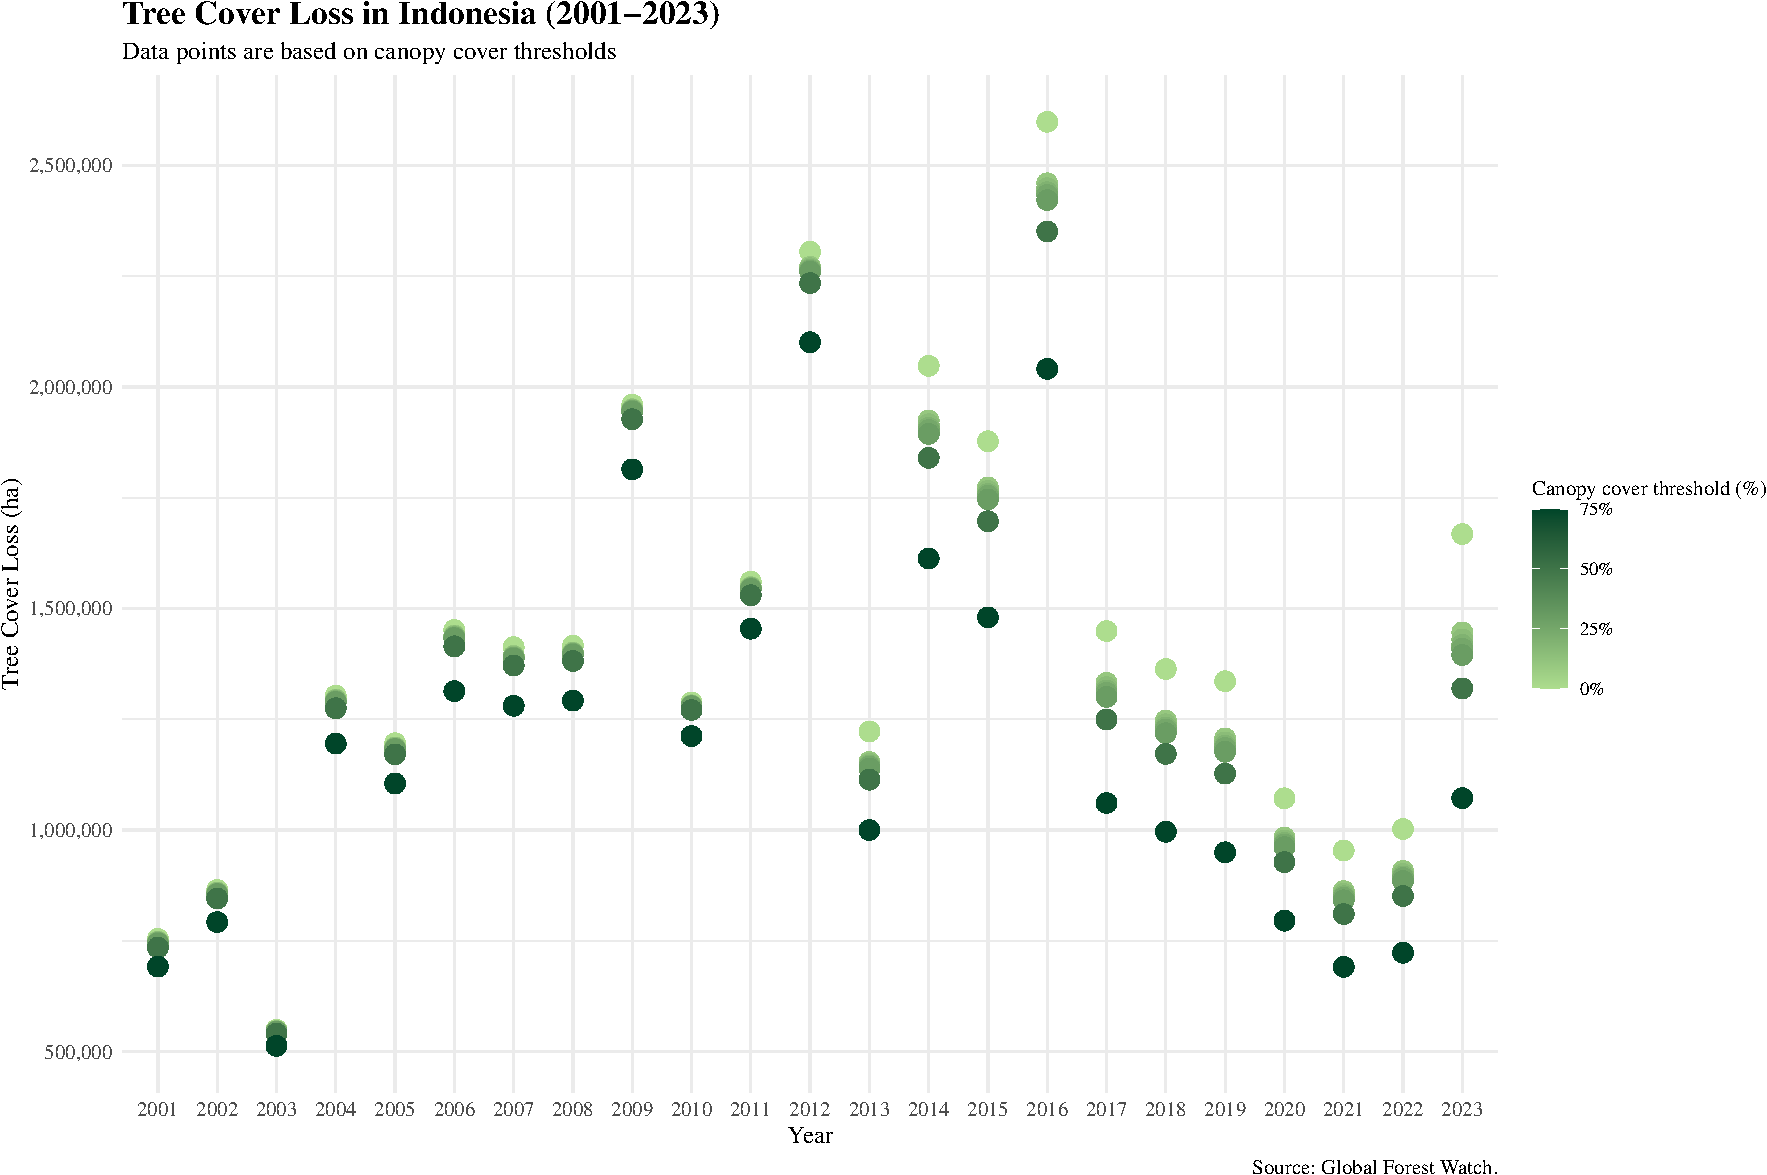
\includegraphics{index_files/figure-latex/unnamed-chunk-3-1.pdf}

\begin{Shaded}
\begin{Highlighting}[]
\FunctionTok{dir.create}\NormalTok{(}\StringTok{"Figures"}\NormalTok{)}
\FunctionTok{ggsave}\NormalTok{(}\AttributeTok{filename =} \StringTok{"Figures/country\_tc\_loss\_figure.jpg"}\NormalTok{)}
\end{Highlighting}
\end{Shaded}

\subsubsection{Analysis \& Results for Question Statement
1}\label{analysis-results-for-question-statement-1}

The highest tree cover loss occurred in 2016, 2012, and 2008,
respectively. In 2016, areas with 0\% canopy threshold experienced the
most loss compared to areas in the 25-75\% canopy cover. There was a
significant reduction in tree cover loss from 2016 to 2017, followed by
a gradual decrease until 2022, after which there was a surge of loss in
2023.

\subsubsection{Question statement 2}\label{question-statement-2}

*** What are the magnitudes of tree cover loss per year in each province
from 2001 to 2023?***

I chose to create a line graph where each line corresponds to a province
in Indonesia. However, the presence of 33 provinces may result in
overlapping lines, making it difficult to distinguish each one.
Therefore, I opted to make an interactive plot so that viewers can hover
over the lines to see the year, province, and amount of tree cover loss.
This interactive plot allows viewers to explore specific provinces by
clicking their names in the legend or compare multiple provinces at
once.

\begin{Shaded}
\begin{Highlighting}[]
\FunctionTok{library}\NormalTok{(plotly)}

\CommentTok{\#make the canvas}
\NormalTok{subnational\_tcloss\_plot }\OtherTok{\textless{}{-}} \FunctionTok{ggplot}\NormalTok{(}\AttributeTok{data =}\NormalTok{ filtered\_subnational\_tc\_loss, }\AttributeTok{mapping =}
         \FunctionTok{aes}\NormalTok{(}\AttributeTok{x =}\NormalTok{ year\_tc\_loss, }\AttributeTok{y =}\NormalTok{ tc\_loss, }\AttributeTok{group =} 
\NormalTok{               subnational1, }\AttributeTok{color =}\NormalTok{ subnational1, }\AttributeTok{text =} \FunctionTok{paste0}\NormalTok{(}\StringTok{"Year: "}\NormalTok{, year\_tc\_loss,}
              \StringTok{"\textless{}br\textgreater{}Tree Cover Loss: "}\NormalTok{, tc\_loss, }
              \StringTok{"\textless{}br\textgreater{}Region: "}\NormalTok{, subnational1)))  }

\CommentTok{\#add the details and create customisation}
\NormalTok{p }\OtherTok{\textless{}{-}}\NormalTok{ subnational\_tcloss\_plot }\SpecialCharTok{+} \FunctionTok{geom\_line}\NormalTok{() }\SpecialCharTok{+} \FunctionTok{geom\_point}\NormalTok{() }\SpecialCharTok{+}
  \FunctionTok{labs}\NormalTok{(}\AttributeTok{x =} \StringTok{"Year"}\NormalTok{, }\AttributeTok{y =} \StringTok{"Tree Cover Loss (ha)"}\NormalTok{,}
       \AttributeTok{title =} \StringTok{"Tree Cover Loss Indonesia by Province (2001{-}2023)"}\NormalTok{,}
       \AttributeTok{subtitle =} \StringTok{"Data points are based on canopy cover threshold of 30\%"}\NormalTok{,}
       \AttributeTok{caption =} \StringTok{"Source: Global Forest Watch."}\NormalTok{, }\AttributeTok{color =} \ConstantTok{NULL}\NormalTok{) }\SpecialCharTok{+}
  \FunctionTok{theme\_minimal}\NormalTok{() }\SpecialCharTok{+} \FunctionTok{scale\_y\_continuous}\NormalTok{(}\AttributeTok{labels =}\NormalTok{ scales}\SpecialCharTok{::}\NormalTok{comma) }\SpecialCharTok{+}
\NormalTok{  (}\FunctionTok{theme}\NormalTok{(}\AttributeTok{plot.title =} \FunctionTok{element\_text}\NormalTok{(}\AttributeTok{family =} \StringTok{"Times"}\NormalTok{, }\AttributeTok{size =} \DecValTok{16}\NormalTok{, }\AttributeTok{face =} \StringTok{"bold"}\NormalTok{),}
         \AttributeTok{plot.subtitle =} \FunctionTok{element\_text}\NormalTok{(}\AttributeTok{family =} \StringTok{"Times"}\NormalTok{, }\AttributeTok{size =} \DecValTok{12}\NormalTok{),}
         \AttributeTok{axis.title =} \FunctionTok{element\_text}\NormalTok{(}\AttributeTok{family =} \StringTok{"Times"}\NormalTok{, }\AttributeTok{size =} \DecValTok{12}\NormalTok{),}
         \AttributeTok{axis.text =} \FunctionTok{element\_text}\NormalTok{(}\AttributeTok{family =} \StringTok{"Times"}\NormalTok{, }\AttributeTok{size =} \DecValTok{8}\NormalTok{), }
         \AttributeTok{plot.caption =} \FunctionTok{element\_text}\NormalTok{(}\AttributeTok{family =} \StringTok{"Times"}\NormalTok{, }\AttributeTok{size =} \DecValTok{10}\NormalTok{),}
         \AttributeTok{legend.title =} \FunctionTok{element\_text}\NormalTok{(}\AttributeTok{family =} \StringTok{"Times"}\NormalTok{, }\AttributeTok{size =} \DecValTok{10}\NormalTok{),}
         \AttributeTok{legend.text =} \FunctionTok{element\_text}\NormalTok{(}\AttributeTok{family =} \StringTok{"Times"}\NormalTok{, }\AttributeTok{size =} \DecValTok{8}\NormalTok{)))}

\FunctionTok{ggsave}\NormalTok{(}\AttributeTok{filename =} \StringTok{"Figures/subnational\_figure1.jpg"}\NormalTok{, }\AttributeTok{plot =}\NormalTok{ p)}


\CommentTok{\#create interactive plot}
\NormalTok{interactive\_plot }\OtherTok{\textless{}{-}} \FunctionTok{ggplotly}\NormalTok{(p, }\AttributeTok{tooltip =} \StringTok{"text"}\NormalTok{)}
\NormalTok{interactive\_plot}

\FunctionTok{library}\NormalTok{(htmlwidgets)}
\FunctionTok{saveWidget}\NormalTok{(interactive\_plot, }\StringTok{"Figures/subnational\_tcloss\_plot.html"}\NormalTok{)}
\end{Highlighting}
\end{Shaded}

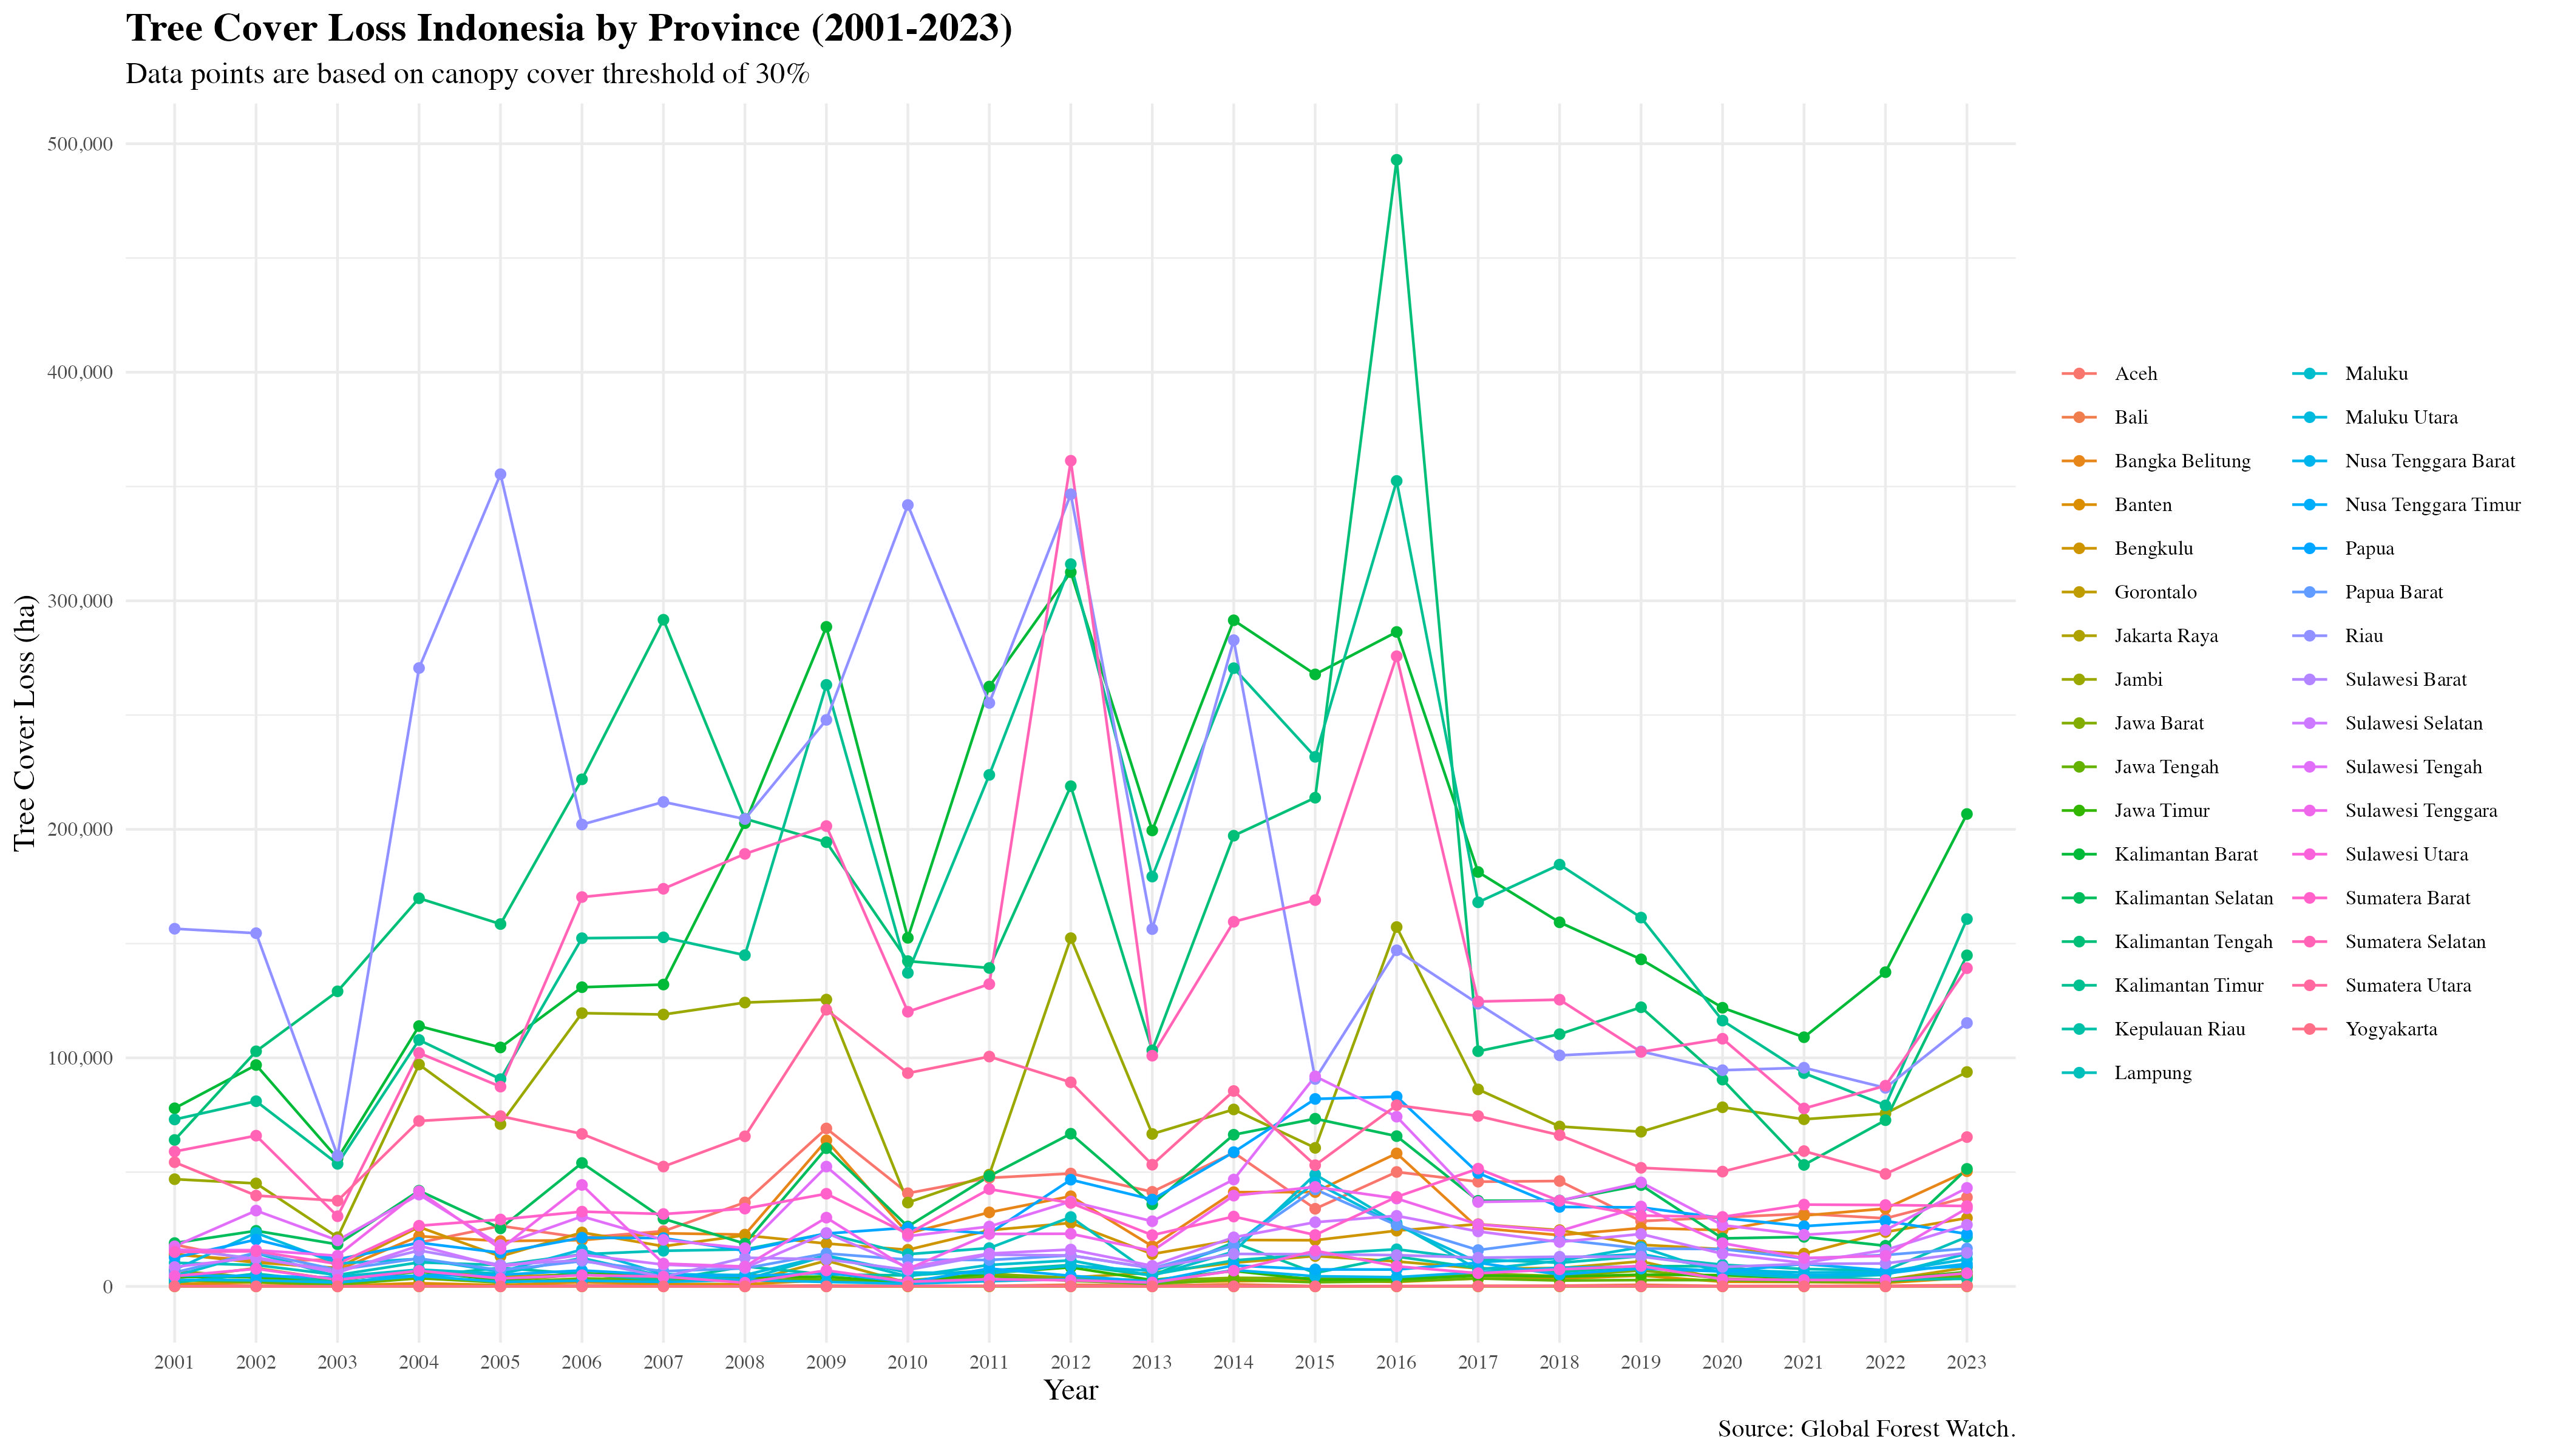
\includegraphics{Figures/subnational_figure1.jpg}

\subsubsection{Analysis \& Results for Question Statement
2}\label{analysis-results-for-question-statement-2}

In the beginning of the 2001--2023 period, Riau had the most tree cover
loss, at 355,415 hectares. A consistent trend was seen between the
scatter plot and the interactive plot, indicating that the highest tree
cover loss occurred in 2016. The interactive plot clearly illustrates
that the loss happened in Kalimantan Tengah, reaching almost 500,000
hectares, followed by Kalimantan Timur at 352,451 hectares and
Kalimantan Barat at 286,373 hectares.

\subsection{Conclusions}\label{conclusions}

Data visualisation shows that both country and subnational datasets
exhibit a similar trend, characterised by an increase in tree loss cover
from 2001 to 2016, followed by a decline until 2022. Plotting the
interactive line graph reveals that regions of Kalimantan Island
experienced the most tree cover loss during the peak in 2016. It is
interesting to see that both country and subnational data show an upward
trend of tree cover loss from 2022 to 2023. These findings raise
questions about why there is another increase after several years of
keeping the losses lower than the 2001--2016 period and what kind of
activity is happening on the Kalimantan island that caused the area to
suffer a high number of tree cover losses.

There should be some caution in interpreting this data. GFW noted that
tree cover loss data does not correspond to deforestation, as this
``loss'' refers to the elimination or death of tree cover that is
attributed to various factors, such as mechanical harvesting, fire,
disease, or storm damage. In addition, changes in methodology and
integration of new satellite data resulted in higher estimates of
``loss'' compared to previous years. Further information on this matter
is available through this link:
\url{https://www.globalforestwatch.org/blog/data-and-research/tree-cover-loss-satellite-data-trend-analysis/}

\subsection{References}\label{references}

Global Forest Watch. (2024). World Resource Institute. Retrieved 26
November 2024, from
\url{https://www.globalforestwatch.org/dashboards/country/IDN?category=land-cover}

Greenpeace. (n.d.) \emph{Indonesian Forests \& Palm Oil}. Retrieved 4
December 2024, from
\url{https://www.greenpeace.org/usa/forests/indonesian-forests-palm-oil/}

Greenpeace Southeast Asia. (2024, November 20). \emph{Papuan Indigenous
Activists Present Quarter-Million Signatures to Supreme Court}.
\url{https://www.greenpeace.org/southeastasia/press/66400/papuan-indigenous-activists-present-quarter-million-signatures-to-supreme-court/}

Hansen, M. C., Potapov, P. V., Moore, R., Hancher, M., Turubanova, S.
A., Tyukavina, A., Thau, D., Stehman, S. V., Goetz, S. J., Loveland, T.
R., Kommareddy, A., Egorov, A., Chini, L., Justice, C. O., \& Townshend,
J. R. G. (2013). High-Resolution Global Maps of 21st-Century Forest
Cover Change. \emph{Science}, 342(6160), 850--853.
\url{https://doi.org/10.1126/science.1244693}

Van Laar, A., \& Akça, A. (2007). \emph{Forest mensuration} (Vol. 13).
Springer Science \& Business Media.

Vatandaslar, C., Lee, T., Bettinger, P., Ucar, Z., Stober, J., \&
Peduzzi, A. (2024). Mapping percent canopy cover using individual tree-
and area-based procedures that are based on airborne LiDAR data: Case
study from an oak-hickory-pine forest in the USA. \emph{Ecological
Indicators}, 167, 112710.
\url{https://doi.org/10.1016/j.ecolind.2024.112710}

Weisse, M., \& Potapov, P. (2021, April 28). \emph{How Tree Cover Loss
Data Has Changed Over Time}. Global Forest Watch.
\url{https://www.globalforestwatch.org/blog/data-and-tools/tree-cover-loss-satellite-data-trend-analysis}

\end{document}
